\documentclass{article}

%=====================================================================
%============================= packages ==============================

%\usepackage{geometry}
\usepackage{amsmath}
\usepackage{amssymb}
\usepackage{stmaryrd}
\usepackage{fancyhdr}
\usepackage{natbib}
\usepackage[normalem]{ulem}
\usepackage{examples-slim}
\usepackage{xcolor}
\usepackage{graphicx}
\usepackage{float}
\usepackage{multirow}
\usepackage{booktabs}
\usepackage{colortbl}
\usepackage{caption}
\usepackage{subcaption}
\definecolor{black}{rgb}{0,0,0}
\usepackage[colorlinks, linkcolor=black, urlcolor=black, citecolor=black]{hyperref}

\bibpunct[; ]{(}{)}{;}{a}{}{,}  % natbib citation style

%=====================================================================
%========================= cross-references ==========================

% Flexible sec/fig/tbl/def cross-refs.
\newcommand{\Secref}[1]{Section~\ref{#1}}
\newcommand{\secref}[1]{section~\ref{#1}}
\newcommand{\dashsecref}[2]{sections~\ref{#1}--\ref{#2}}

\newcommand{\Defref}[1]{Def.~\ref{#1}}
\newcommand{\defref}[1]{def.~\ref{#1}}
\newcommand{\Defrefc}[2]{\Defref{#1}, clause~\ref{#2}}
\newcommand{\defrefc}[2]{\defref{#1}, clause~\ref{#2}}

\newcommand{\Figref}[1]{Figure~\ref{#1}}
\newcommand{\figref}[1]{figure~\ref{#1}}
\newcommand{\dashfigref}[2]{figures~\ref{#1}--\ref{#2}}
\newcommand{\Tabref}[1]{Table~\ref{#1}}
\newcommand{\tabref}[1]{table~\ref{#1}}

% Examples:
\newcommand{\eg}[1]{(\ref{#1})}
\newcommand{\subeg}[2]{(\ref{#1}\ref{#2})}
\newcommand{\dblsubeg}[3]{(\ref{#1}\ref{#2},~\ref{#3})}
\newcommand{\dashsubeg}[3]{(\ref{#1}\ref{#2}--\ref{#3})}

% In-text citations
\newcommand{\posscitet}[1]{\citeauthor{#1}'s~(\citeyear{#1})}
\newcommand{\sposscitet}[1]{\citeauthor{#1}'~(\citeyear{#1})}
\newcommand{\possciteauthor}[1]{\citeauthor{#1}'s}
\newcommand{\spossciteauthor}[1]{\citeauthor{#1}'}
\newcommand{\pgposscitet}[2]{\citeauthor{#1}'s~(\citeyear{#1}:~#2)}
\newcommand{\secposscitet}[2]{\citeauthor{#1}'s~(\citeyear{#1}:~$\S$#2)}
\newcommand{\pgcitealt}[2]{\citealt{#1}:~#2}
\newcommand{\seccitealt}[2]{\citealt{#1}:~$\S$#2}
\newcommand{\pgcitep}[2]{(\citealt{#1}:~#2)}
\newcommand{\seccitep}[2]{(\citealt{#1}:~$\S$#2)}
\newcommand{\pgcitet}[2]{\citeauthor{#1}~(\citeyear{#1}:~#2)}
\newcommand{\seccitet}[2]{\citeauthor{#1}~(\citeyear{#1}:~$\S$#2)}

%=====================================================================
%============================ text styles ============================

\newcommand{\word}[1]{\emph{#1}}
\newcommand{\tech}[1]{\textbf{#1}}
\definecolor{maroon}{HTML}{990000}
\newcommand{\highlight}[1]{{\color{maroon}#1}}

%=====================================================================
%============================== judgments ============================

\newcommand{\bad}{\sqz{${}^\ast$}}
\newcommand{\freebad}{${}^\ast$}
\newcommand{\marked}{\sqz{${}^\#$}}
\newcommand{\freemarked}{${}^\#$}

%=====================================================================
%=============================== model ===============================


\newcommand{\tuple}[1]{\ensuremath{\left< #1 \right>}}
\newcommand{\set}[1]{\ensuremath{\left\{ #1 \right\}}}
\newcommand{\True}{\texttt{T}}
\newcommand{\False}{\texttt{F}}
\newcommand{\Reals}{\mathbb{R}}
\newcommand{\given}{\mid}
\newcommand{\Indicator}{\mathbb{I}}

\newcommand{\sem}[1]{\ensuremath{\llbracket#1\rrbracket}}
\newcommand{\States}{W}
\newcommand{\state}{w}
\newcommand{\Lex}{\mathcal{L}}
\newcommand{\LexStar}{\Lex^{\ast}}
\newcommand{\LexSet}{\mathbf{L}}
\newcommand{\Messages}{M}
\newcommand{\msg}{m}
\newcommand{\Costs}{C}
\newcommand{\Prior}{P}
\newcommand{\LexPrior}{P_{\LexSet}}

\newcommand{\listenerZero}{l_{0}}
\newcommand{\speakerOne}{s_{1}}
\newcommand{\listenerOne}{l_{1}}
\newcommand{\SpeakerK}[1][k]{S_{#1}}
\newcommand{\ListenerK}[1][k]{L_{#1}}

\newcommand{\nullmsg}{\mathbf{0}}

%=====================================================================
%============================ annotations ============================

\let\oldmarginpar\marginpar
\renewcommand{\marginpar}[1]{\oldmarginpar[\color{red}\raggedright\scriptsize #1]{\color{red}\raggedright\scriptsize #1}}

\newcommand{\textnote}[1]{{\color{red}#1}}

%=====================================================================
%============================== colors ===============================

\definecolor{lightgray}{HTML}{CCCCCC} 

\definecolor{highlightcolor}{HTML}{D95F02}
\definecolor{annotationcolor}{HTML}{777777} 
\definecolor{worldinfocolor}{HTML}{E7298A}
\definecolor{lexcolor}{HTML}{D95F02}
\definecolor{costcolor}{HTML}{A6761D}
\definecolor{defcolor}{HTML}{D95F02}
%\definecolor{hurfordcolor}{HTML}{00CC33}
\definecolor{hurfordcolor}{HTML}{1B9E77}
\newcommand{\hurford}[1]{{\relax\color{hurfordcolor}#1}}
\newcommand{\definitional}[1]{\relax{\color{defcolor}#1}}

\newcommand{\graycell}[1]{{\cellcolor[gray]{.8}#1}}

%=====================================================================
%============================== helpers ==============================

\newcommand{\porq}{p\,\word{or}\,q}
\newcommand{\pandq}{p\,\&\,q}

\newcommand{\disjlexicon}[2]{
  \left[
    \begin{array}[c]{l@{ \ \mapsto \ } l}
      \porq    & \set{#1} \\
      \pandq   & \set{#2} \\
      \nullmsg & \set{w_{1}, w_{2}, w_{3}} \\
    \end{array}
  \right]}

\newcommand{\listenerMatrix}[6]{
  \begin{array}[c]{l *{4}{r}}
    \toprule
    #1 & w_{1} & w_{2} & w_{3} \\
    \midrule
    p        & #2 \\
    q        & #3 \\              
    \pandq   & #4 \\
    \porq    & #5 \\
    \nullmsg & #6 \\
    \bottomrule
  \end{array}}

\newcommand{\speakerMatrix}[4]{
  \begin{array}[c]{r *{5}{r}}
    \toprule
    #1 & p & q & \pandq & \porq & \nullmsg \\
    \midrule
    w_{1} & #2 \\
    w_{2} & #3 \\ 
    w_{3} & #4 \\ 
    \bottomrule
  \end{array}}

\newcommand{\ListenerKMatrix}[4]{
  \begin{array}[c]{l *{3}{r}}
  \toprule
    #1 & w_{1} & w_{2} & w_{3} \\
    \midrule
    \LexStar  & #2 \\
    \Lex_{1}  & #3 \\
    \Lex_{2}  & #4 \\
    \bottomrule
  \end{array}}

\newcommand{\SpeakerKMatrix}[4]{
  \begin{array}[c]{l *{3}{r}}
    \toprule
    \Lex_{#1} & \porq & \pandq & \nullmsg \\
    \midrule
    w_{1}  & #2 \\
    w_{2}  & #3 \\
    w_{3}  & #4 \\
    \bottomrule
  \end{array}}

\newcommand{\smalldisjlex}[3]{
  \setlength{\arraycolsep}{1pt}
  \left[
    \begin{array}[c]{l@{ \ \mapsto \ }r@{, \ } l@{ \ \mapsto \ }r@{, \ } l@{ \ \mapsto \ }r}
      A & \set{#1} &
      B & \set{#2} &
      X & \set{#3}
    \end{array}
  \right]}

\newcommand{\smalldisjlexTargetDef}{\smalldisjlex{\definitional{\mathbf{w_{1}}}}{w_{2}}{\definitional{\mathbf{w_{1}}}}}

\newcommand{\smalldisjlexTargetHuford}{\smalldisjlex{\hurford{\mathbf{w_{1}}}}{w_{2}}{\hurford{\mathbf{w_{2}}}}}

\definecolor{highlightcolor}{HTML}{D95F02}
\definecolor{annotationcolor}{HTML}{777777} 
\definecolor{worldinfocolor}{HTML}{E7298A}
\definecolor{lexcolor}{HTML}{D95F02}
\definecolor{costcolor}{HTML}{A6761D}
\definecolor{defcolor}{HTML}{D95F02}
\definecolor{hurfordcolor}{HTML}{00CC33}
\newcommand{\hurford}[1]{{\relax\color{hurfordcolor}#1}}
\newcommand{\definitional}[1]{\relax{\color{defcolor}#1}}

\definecolor{lightgray}{HTML}{CCCCCC} 
%\renewcommand{\graycell}[1]{\colorbox{lightgray}{#1}}
\newcommand{\whitecell}[1]{\colorbox{white}{#1}}

\newcommand{\lismat}[4]{
  \setlength{\arraycolsep}{1pt}
  \begin{array}[c]{l *{3}{r}}
    \toprule
    #1 & w_{1} & w_{2} & w_{1}{\vee}w_{2} \\
    \midrule
    A & #2\\
    X & #3 \\
    A\,\word{or}\,X & #4 \\
    \bottomrule
  \end{array}}

\newcommand{\spkmat}[4]{
  \setlength{\arraycolsep}{1pt}
  \begin{array}[c]{l *{3}{r}}
    \toprule
    #1 & A & X & A\,\word{or}\,X \\
    \midrule
    w_{1} & #2\\
    w_{2} & #3 \\
    w_{1}{\vee}w_{2} & #4 \\
    \bottomrule      
  \end{array}}                   

\renewcommand{\disjlexicon}[2]{
  \renewcommand{\arraystretch}{1}
  \left[   
    \begin{array}[c]{l@{ \ \mapsto \ } l}
      p   & \set{#1} \\
      q  & \set{#2} \\
    \end{array}
  \right]}

\newcommand{\closurelex}[6][1]{
  \renewcommand{\arraystretch}{1}
  \begin{array}[c]{*{8}{r}}
    \toprule
    &w_{1}&w_{2}&w_{3}&w_{1}{\vee}w_{2}&w_{1}{\vee}w_{3}&w_{2}{\vee}w_{3}&w_{1}{\vee}w_{2}{\vee}w_{3}\\
    \midrule
    p      & #2 \\
    q      & #4 \\
    \pandq & #3 \\
    \porq  & #5 \\
    \nullmsg & #6 \\
    \bottomrule
  \end{array}}


\begin{document}

%%%%%%%%%%%%%%%%%%%%%%%%%%%%%%%%%%%%%%%%%%%%%%%%%%%%%%%%%%%%%%%%%%%%%%

\title{Negotiating lexical uncertainty and expertise with disjunctive utterances}
\author{Roger Levy and Christopher Potts}
\maketitle

%%%%%%%%%%%%%%%%%%%%%%%%%%%%%%%%%%%%%%%%%%%%%%%%%%%%%%%%%%%%%%%%%%%%%%

\section{Communicating in language about language}\label{sec:introduction}

Natural languages are neither fixed across time nor identically
reproduced in all speakers, but rather continually renegotiated during
interactions \citep{Clark97}. Discourse participants accommodate to
each other's usage patterns \citep{Giles:Coupland:Coupland:1991}, form
temporarily lexical pacts to facilitate communication
\citep{Clark:Wilkes-Gibbs:1986,Brennan:Clark:1996}, and instruct each
other about their linguistic views. Some of this communication in
language about language is direct, as with explicit definitions like
\word{`oenophile' means wine lover}, but much of it arrives via
secondary pragmatic inferences, as when \word{X such as Y} conveys
that \word{X} subsumes \word{Y} \citep{Hearst92,SnowEtAl05}.

Disjunction supports what appear to be opposing inferences about
language. On the one hand, \word{X or Y} tends to convey that the
meanings of \word{X} and \word{Y} are presumed to be disjoint
\citep{Hurford:1974}, because the speaker holds such a view of the
lexicon or is worried that the listener might. This pressure to
exclusivize is robust enough to overcome even seemingly non-negotiable
aspects of the lexicon; a medical webpage warns ``If you still have
symptoms or severe blockage in your arteries, you may need angioplasty
or surgery'', sending a clear signal that angioplasty and surgery
are distinct options. Its continuation presupposes just that: 
``Having one of these procedures may save your leg''. The disjunction
might seem to be a needlessly verbose way of conveying the meaning of
the more general disjunct, but the costs could be worth paying in
virtue of the lexical side-effect of exclusivization.

On the other hand, disjunctions like \word{wine lover or oenophile}
can be used to convey that the two disjuncts are roughly synonymous
\citep{Horn89}, thereby providing secondary information that maximally
violates the pressure to exclusivize. This inference is more rarefied
than the exclusivization inference, but it can arise in a broad range
of contexts in which such definitional or identificational information
has social or communicative value. It is striking that the
definitional and exclusivization inferences are supported by a single
lexical item, and the puzzle deepens when we see that the empirical
picture is not a quirk of English, but rather one that we find in a
wide range of typologically and geographically diverse languages.

In this paper, we capture both of these classes of inference within a
single recursive Bayesian model of pragmatic reasoning. The model
finds its conceptual origins in \posscitet{Lewis69} work on signaling
systems and builds on ideas from iterated best response models
\citep{Jaeger:2007,Jaeger:2011,Franke09DISS} and more thoroughly
probabilistic variants of them
\citep{CamererHo:2004,Frank:Goodman:2012}. The crucial feature of our
model is that it lets discourse participants communicate, not just
about the world, but also about the language they are using
\citep{Bergen:Goodman:Levy:2012,bergen-levy-goodman:2014}: the
speaker's intentions in production are characterized in terms of both
world information and linguistic information, and the listener's
pragmatic reasoning is cast as a problem of joint inference about the
speaker's intended meaning and preferred lexicon
\citep{Smith:Goodman:Frank:2013}. We show that, within this model,
both exclusivization and definitional inferences arise naturally from
the expected semantic content of disjunction, depending on contextual
parameters relating to speaker expertise, listener malleability, and
information contained in the common ground. The model thus offers a
genuinely pragmatic account of these inferences as well as
characterizations of their stability and their communicative value.

%%%%%%%%%%%%%%%%%%%%%%%%%%%%%%%%%%%%%%%%%%%%%%%%%%%%%%%%%%%%%%%%%%%%%%

\section{Lexical side-effects from disjunction}\label{sec:data}

This section offers more expanded characterizations of the
exclusivization and definitional uses of disjunction. We seek to
identify features of the contexts of use, and the resulting
inferences, that are shared across the two, and to begin to pinpoint
the features of the context that steer speakers and listeners toward
one or the other. These findings inform the modeling we describe in
\dashsecref{sec:model}{sec:analysis}.


%=====================================================================

\subsection{Hurfordian effects}\label{sec:data:overlapping}

\posscitet{Hurford:1974} generalization (HG) is a direct statement of
the overall communicative pressure to treat disjuncts as exclusive:
%
\begin{examples}
\item\label{hg}%
  ``The joining of two sentences by \word{or} is unacceptable if one
  sentence entails the other; otherwise the use of \word{or} is
  acceptable.'' (p.~410)
\end{examples}
%
The generalization is stated in terms of sentences, but Hurford's
examples, given in \eg{hex} with his original judgments, make it clear
that he intends it to hold for sub-sentential disjuncts as well (he is
likely assuming conjunction reduction):
%
\begin{examples}
\item\label{hex}
  \begin{examples}
  \item Ivan is an American or Russian.
  \item The painting is of a man or a woman.
  \item The value of $x$ is greater than or equal to 6.
  \item\label{ex-bad1}\bad John is an American or Californian.
  \item\label{ex-bad2}\bad The painting is of a man or a bachelor.
  \item\label{ex-bad3}\bad The value of $x$ is greater than or not equal to 6.
  \end{examples}
\end{examples}

\citeauthor{Hurford:1974} uses HG to probe the nature and distribution
of conversational implicatures (see also
\citealt{Gazdar79b,ChierchiaFoxSpector08}), and \citet{Singh:2008}
extends it to cases in which the disjuncts are merely overlapping. We
endorse the guiding insight behind these accounts but reject the
assumption that HG violations reliably lead to, or even correlate
with, unacceptability or ungrammaticality. Disjunctions of apparently
entailing phrases are routine; all of the examples marked as
ungrammatical in \eg{hex} are easy to find in fluent English text on
the Web:
%
\begin{examples}
\item\label{hex-good}
  \begin{examples}
  %\item ``How much does the average american or californian pay every
  %  year toward state taxes?''
  \item ``\ldots and we trust that some of our American or Californian
    friends will tell us something of its growth of flower and fruit
    in its native habitats''
  \item ``It doesn't matter if you ask a boy or a man or a bachelor or
    even a husband, \ldots''
  \item ``the effect was greater than, or not equal to, the cause.''
  \end{examples}
\end{examples}

We have collected a large corpus of apparent counterexamples,
available at \url{http://goo.gl/VAGqnB}. Here is a small sample from
that corpus:
%
\begin{examples}
\item\label{ourcorpus} 
  %
  \begin{examples}
    %%%%%%%%%% X < Y
  \item Stop discrimination of an \highlight{applicant or person} due
    to their tattoos.
  \item Promptly report any \highlight{accident or occurrence}.
  \item The anchor will lie on the bottom and the \highlight{canoe or
      boat} will be held by the stream's current.
  \item ``As an \highlight{actor or performer}, you are always worried
    about what the next job's going to be,'' Hensley says.
    %%%%%%%%%%  X > Y
  \item After the loss of the \highlight{animal or pet}, there are
    further coping strategies available for the grieving individual.
  \item Bush was captured slyly removing \highlight{a candy or gum}
    from his mouth.
  \item Heroic is not a word one uses often without embarrassment to
    describe a \highlight{writer or playwright} \ldots
  \item But he never attended school during his senior year, never
    attended a \highlight{party or prom}.
  \end{examples}
\end{examples}
%
The dataset includes XXXX cases where the left disjunct entails the
right, and XXXX in which the right entails the left.  In addition, we
conjecture that, for any two nouns $N_{1}$ and $N_{2}$ one believes to
be in an overlap or proper entailment relation, a Web search for
``$N_{1}$ or $N_{2}$'' will generally yield counterexamples, as will
``$N_{2}$ or $N_{1}$''. 

\marginpar{Perhaps conduct and footnote an N-grams experiment on place names.}

Of course, one would like to have a more rigorous sampling procedure,
to evaluate the prevalance of these disjunctions and to probe ordering
preferences that might relate to the direction of entailment. However,
we do not see a way to do this accurately. The primary obstacle is, we
believe, an important property of the phenomenon itself: judgments
about lexical entailment are inherently very messy because of the
flexible ways in which people refine meanings in context. As a result,
there often isn't a single objective answer to the question of whether
two disjuncts stand in an an entailment
relation. Example~\eg{churchorsynagogue} illustrates:
%
\begin{examples}
\item\label{churchorsynagogue} ``In 1940, 37 percent of us had gone to
  a church or synagogue in the last week.''
\end{examples}
%
Some speakers have firm judgments that \word{church} and
\word{synagogue} exclude each other, making this case clearly
HG-respecting. However, it is easy to find uses of the phrase
``synagogues and other churches'', which presuppose that a synagogue
is a kind of church. The important thing for our purposes is that the
insight behind HG shines through this uncertainty: no matter what
one's initial view of the lexicon is, disjunctions like \word{church
  or synagogue} make salient a view of the lexicon in which the terms
are semantically disjoint. The speaker will be perceived as endorsing
such a view, at least for the current conversational exchange, and the
listener can either adopt that assumption or push back.

This lexical uncertainty motivates our own explanation for why
speakers utter HG-violating disjunctions. In broad terms, we say that
such examples convey that the speaker is treating the two terms as
exclusive. There are many potential motivations for this. Perhaps the
most mundane is that the speaker simply lexicalizes the two terms as
exclusive. The disjunction is likely to be easily justified in such
cases, as it might be the most efficient and direct way of identifying
the union of the two terms.

\marginpar{Perhaps report on our attempt to reproduce Chemla's result.}

More interesting are cases in which the speaker's disjunction seems to
be part of an attempt to manage the listener's inferences. For
instance, the speaker who uses the phrase \word{swimwear or bikini}
might be concerned that using \word{swimwear} alone will trigger an
ad-hoc scalar implicature \citep{Hirschberg85} excluding the salient
subkind of bikinis. \citet{Chemla-HurfordCounts} studies this class of
inferences, presenting suggestive evidence that the frequency of
disjunctions \word{X or Y} is positively correlated with the
likelihood that \word{X} converstionally implicates \word{not Y} as
estimated by the experimental results of \citet{vanTiel-etal:2013}.
Similarly, the speaker might be seeking to block an implicature that a
general term is \emph{limited to} a prototypical subkind
\citep{Levinson00}. For example, where \word{boat} tends to identify
motorboats, the speaker might use \word{boat or canoe} to ensure that
canoes are included.  In both of these cases, the speaker is concerned
that the general term \word{X} will be construed as
$\sem{\word{X}}-\sem{\word{Y}}$ for some \word{Y}. Thus, \word{X} or
\word{Y} is a hedge against the possibility that the listener's view
of language is such that, at least in the current context,
$\sem{\word{X}} \cap \sem{\word{Y}} = \emptyset$, or, as in
\posscitet{Singh:2008} account,
$\sem{\word{Y}} \nsubseteq \sem{\word{X}}$.

The above situations place the speaker in a defensive position. Her
own lexicon might allow her to use just the general term to convey her
intentions, but she is concerned that the listener will arrive at a
different conclusion. The costs of disjunction are therefore worth
paying even if it adds no new information given the speaker's lexicon.
However, the speaker can play a more active role as well, using
disjunctions to instruct the listener about the right lexicon. Our
\secref{sec:introduction} example containing ``you may need
angioplasty or surgery'' seems to be an instance of this: the
disjunction conveys secondary information that \word{angioplasty} and
\word{surgery} will be treated as separate options in the current
discourse. If HG were adopted as an explicit theoretical constraint,
then the possibility of doing this would more or less follow --- we
just require the additional premise that the listener is charitable
and so will try to find an acceptable construal of the utterance. The
model we develop in \secref{sec:model} also supports this kind of
reasoning, but it requires no independent statement of HG.
 
%%%%%%%%%%%%%%%%%%%%%%%%%%%%%%%%%%%%%%%%%%%%%%%%%%%%%%%%%%%%%%%%%%%%%%

\subsection{Definitional effects}\label{sec:data:definitional}

% A Geological History of Manhattan or New York

Definitional uses of disjunction like \word{wine lover or oenophile}
seem to be rarer and more contextually restricted even than the
somewhat unusual compatible and subsumptive disjunctions reviewed
above. We know they are attested in Chinese, Finnish, German, Hebrew,
Ilokano, Japanese, Russian, and Tagalog, suggesting that, despite
their specialized nature, they represent a principled extension of the
standard uses of disjunction.

The definitional meaning is secondary to the central message --- a
sort of side-effect of the main utterance. This contrasts with overt
definitions like \word{oenophile means `wine-lover'} or
\word{oenophile: wine-lover} (in a dictionary context). Our model
captures this by characterizing the definitional effect as an
inference about the lexicon, rather than about the information
conveyed. Alternative forms achieving the same thing: apposition
\word{oenophile (`wine-lover')}. There might be others. Apposition
would seem to have a conjunctive semantics (broadly speaking), so it
is striking that there seem not to be definitional uses of conjunction
itself.

Definitional readings need not be perfectly definitional in the sense
of complete, pure synonymy. Indeed, it is likely that no definition
achieves this ideal, especially if connotational meaning is
included. (Examples: \word{internet or computer network}, and even our
wine-lover example, where \word{oenophile} seems to elevate the
concept to something more refined than \word{wine lover} picks out.)

Definitional readings arise most easily when the speaker is mutually
and publicly known to be a expert in the domain covered by the terms
and the listener is mutually and publicly known to be inexpert in that
area. In such cases, the speaker can use the disjunction to convey
secondary definitional information. However, other contexts also
support such readings. In some naturalistic uses, definitional
disjunction is also seen when it is not common ground that the
listener doesn't know the novel term, but rather when there is value
for the speaker in demonstrating knowledge of the novel term's
meaning.  We suggest that these uses are derivative of the core usage
that we have presented a model of.

The listener might use a definitional disjunction to convey expertise
indirectly (without asserting it directly) --- an ambitious
undergraduate conveying competence to a professor, for example. In
other cases, the speaker and listener might both be experts in the
domain and see a value (jointly or just in the current speaker's eyes)
of using a word in a specialized sense in order to name a concept
efficiently. In such cases, since the definition is not asserted or
given overtly, but rather inferred, we would expect it to have to be a
relatively normal sort of adjustment. One would not use it to define a
totally novel word, as in \word{an X or `glomp'}, but one might use it
if the intentions are transparent given the new word's shape \word{a
  solar-powered generator or `sologen'} or th eadjustment is minor and
uncontroversial \word{snobish wine lover or `oenophile'}.

For these reasons, we retreat to a more basic characterization: the
discourse participants must have an interest in communicating about
their language and arriving at a refined, perhaps context-specific
joint understanding of it. In addition, we hypothesize that the cost
of using a disjunction must be fairly small all things considered,
else it is hard to see how the speaker could justify using a
disjunction \word{X or Y} to convey simply $\sem{\word{X}}$.


Overt signals: ad hoc prosody, italics, quotation marks. There is
clearly great pressure to signal definitional readings, though it is
not an absolute requirement.


There can be uncertainty about whether the listener should regard the
disjunction as definitional. We might enter into a blury area in which
the listener is struggling to figure out whether the intentions are
definitional or exclusivizing. This can persist even when one of the
words is unknown to the listener. In such cases, the disjunctive
meaning is just extremely general and will not do justice to the
speaker's intentions.


%%%%%%%%%%%%%%%%%%%%%%%%%%%%%%%%%%%%%%%%%%%%%%%%%%%%%%%%%%%%%%%%%%%%%%

\section{A model of communication with anxious experts}\label{sec:model}

The model finds its conceptual origins in \posscitet{Lewis69} work on
signaling systems and builds on ideas from the iterated best response
models of \citet{Jaeger:2007,Jaeger:2011} and
\citet{Franke09DISS}. Models of this form have been shown to achieve
tight correlations with experimental data (e.g.,
\citealt{Frank:Goodman:2012}) and to offer unified, precise account of
a wide range of conversational implicatures
\citep{bergen-levy-goodman:2014}.

\begin{examples}
\item\label{model}
  \begin{examples}
  \item\label{states}%
    $\States$ is a set of states (worlds, referents, propositions, etc.).
  \item\label{messages}%
    $\Messages$ is a set of messages containing designated `null' message $\nullmsg$.
  \item\label{lex}%
    $\Lex: \Messages \mapsto \wp(\States)$ is a semantic interpretation function. 
    $\Lex'(\nullmsg) = \States$
  \item\label{prior}%
    $\Prior : \States \mapsto [0,1]$ is a prior probability
    distribution over states.    
  \item\label{costs}%
    $\Costs : \Messages \mapsto \Reals$ is a cost function on messages.
    $\Costs(\nullmsg) > \Costs(\msg), {\forall \msg \in \Messages{-}\set{\nullmsg}}$
  \item\label{lexset}%
      $\LexSet = \set{\Lex' : \Lex'(\nullmsg) = \States \text{ and } 
      \forall \msg \in \Messages{-}\set{\nullmsg}, 
      \Lex'(\msg) \neq \emptyset \text{ and } 
      \Lex'(\msg) \subseteq \Lex(\msg)}$
  \item\label{LexPrior}% 
    $\LexPrior : \LexSet \mapsto [0,1]$ is a prior
    probability distribution over lexica.
  \item\label{temps}%
    Real-valued learning-rate parameters $\alpha$, $\beta$, and
    $\gamma$
  \end{examples}
\end{examples}

Clauses~\dashsubeg{model}{states}{costs} define a signaling system. We
imagine that the speaker and listener are playing a game in which the
speaker privately observes a state $\state \in \States$ and produces a
message $\msg \in \Messages$ on that basis, given the context defined
by the signaling system. The listener then uses $\msg$ to guess a
state $\state' \in \States$, and the communication succeeds just in
case $\state = \state'$.

We assume that the set of messages includes a designated null message
$\nullmsg$ that is true in all states in all lexica. It can be thought
of as a catcha-all for the numerous messages in the language that are
not discriminating in the context defined by the signaling system.  No
matter how big and complex our examples grow, we assume that such a
message is always justified. It also helps ensure that various
calculations in the model are well-defined \citep{Jaeger:2011}.

Throughout this basic game, the two players assume that the lexicon is
fixed and mutually, publicly known. In \subeg{model}{lexset}, we see a
first retreat from this assumption. There, we define a set of
refinements of the origianl $\Lex$. In a sense, this defines the space
of pragmatic enrichment allowed by the fixed conventions. Here, we
restrict the lexica to that are refinements of the orginal and assign
non-empty denotations to every message. This is not a deep assumption
of the model, though. One could, for instance, define a much larger
space of lexica and then use the prior $\LexPrior$ to structure
that space with respect to the agents we define just below.

The parameters in \subeg{model}{temps} control the relative weighting
of information about the world, information about the lexicon, and
information about the message costs. We further explicate these
parameters when defining our agents just below.


Our model defines an intuitive hierarchy of agents. The most basic are
$\listenerZero$, $\speakerOne$, and $\listenerOne$. These agents
reason in terms of a fixed lexicon $\Lex$, which, for our purposes,
can be thought of as a standard interpretation function. 

The starting point is $\listenerZero$. This agent simply turns $\Lex$
into a probabilistic formulation that can be used for decision making
in the presence of communucative indeterminacy. The first term just
defines an even distribution over all of the true states $\state$ for
the given message $\msg$, and the second term incorporates the
contextual prior distribution over states $\Prior$.

\begin{examples}
\item\label{l0}%
    $\listenerZero(\state \given \msg, \Lex) \propto
    \frac{\Indicator(\state \in \Lex(\msg))}{|\Lex(\msg)|}
    \Prior(\state)$
\end{examples}

This agent is pragmatic only insofar as it incorporates the contextual 
prior into (a distribution derived from) the truth conditions. Richer
pragmatic inferences start to emerge as soon as we envision a speaker
who can reason in terms of this listener and plan its utterances 
accordingly. The minimal such speaker is $\speakerOne$, which is 
defined recursively in terms of $\listenerZero$:
%
\begin{examples}
  \item\label{s1}% 
    $\speakerOne(\msg \given \state, \Lex) \propto
    \exp
    \left(
      \log\left(\alpha\,\listenerZero(\state \given \msg, \Lex) \right)
      - 
      \gamma\,\Costs(\msg)
    \right)$
\end{examples}
%
Ths definition is a bit cumbersome because of the need to ensure that
all values are positive. At its heart this agent is parallel to
$\listenerZero$ in that it combines a conditional distribution and a
piece of contextual information --- now costs on messages. The result
is a distribution that one can imagaine serving as the basis for
decision making: given that the agent would like to convey that a
certain state holds, which message will do that most effectively for
the listener? The two positive, real-valued parameters $\alpha$ and
$\gamma$ control the rate of learning, in a manner similar to
temperature parameters in reenforcement learning models.

The first pragmatic listener is $\listenerOne$. It is parallel to
$\listenerZero$ except that it reasons, not in terms of the original
lexicon, but rather in terms of $\speakerOne$ reasining about
$\listenerZero$ reasoning about the lexicon:
%
\begin{examples}
  \item\label{l1}% 
    $\listenerOne(\state \given \msg, \Lex) \propto 
    \speakerOne(\msg \given \state, \Lex)
    \Prior(\state)$
\end{examples}

This basic model suffices to derive a range of implicatures involving
context-dependent reasoning about specific terms and their general
counterparts. Broadly speaking, such models can achieve variations on
the theme that using a general term will tend to convey that its
specific counterpart is inappropriate, creating scalar implicatures.
The moadels have been shown to achieve good quantitative fits to
experimental results.  One can also immediately generalize
$\listenerOne$ and $\speakerOne$ to allow them to recursively respond
to each other, which generally has the effect of soldifying
implicatures and predicting new ones that speakers seem less inclined
to perceive \citep{Vogel-etal:2014}.

The generalization we propose is diffent. Rather than defining further
recursion based on these lexicon-specific agents, we now open up the
model to allow for the possibility that the discourse participants are
negotiating not just what information they exchange but also what
language they use to exchange it. Our $\ListenerK$ achieves this on
the listener side; it is based on the social-anxiety listener of
\citet{Smith:Goodman:Frank:2013}.
%
\begin{examples}
  \item\label{Lk}%
    \setlength{\arraycolsep}{2pt}%  
    $\mspace{-4mu}\begin{array}[t]{r c l}
      \ListenerK(\state, \Lex \given \msg) 
      &=&
      \sum_{\Lex \in \LexSet} \listenerOne(\state \given \msg, \Lex) \ListenerK(\Lex \given \msg) 
      \\[1ex]
      \ListenerK(\Lex \given \msg) 
      &\propto& 
      \Prior(\Lex) \sum_{\state\in\States} \SpeakerK(\msg \given \state)\Prior(\state)
    \end{array}$
\end{examples}
%
In terms of its form, the most important feature of this model is that
it makes joint inferences about states and lexica; rather than taking
the lexicon as given, it tries to make guesses about this based on the
speaker's message. The second term models this information
specifically by characterizing the extent to which the speaker's
message discriminates among lexica. This listener is responding to
$\listenerOne$ in sense that it sums over all of the
$\listenerOne(\state\given\msg\Lex)$ inferences for all lexica.
  
Our speaker agent responds to this sophisticated joint listener.  We
assume that the speaker does have a specific lexicon in mind.  More
precisely, this speaker is taken to observe state--lexicon pairs and
produce messages on that basis. In broad terms, it is similar to
$\speakerOne$ except that it includes a new term
$\ListenerK[k-1](\Lex\given\msg)$.

\begin{examples}  
  \item\label{Sk}%
    $\SpeakerK(\msg \given \state, \Lex) \propto 
    \exp
    \left(
      \log
      \left(\alpha\,\ListenerK[k-1](\state \given \msg, \Lex)\right)
      - 
      \beta \log\left(\ListenerK[k-1](\Lex\given\msg)\right)
      -
      \gamma\,\Costs(\msg)
    \right)$
\end{examples}


The above can be unwieldy to think about because of the lexical
inferences. To return to the intuitive picture of simple
state/message signaling, we can sum over lexica, as in 
\eg{lisnorm} and \eg{spknorm}. Both provide useful summaries
of the model's predictions.
%
\begin{examples}
\item\label{lisnorm}% 
  $\ListenerK(\state \given \msg)  = 
  \sum_{\Lex \in \LexSet} \ListenerK(\state, \Lex \given \msg)$
\item\label{spknorm}% 
  $\SpeakerK(\msg \given \state) \propto 
  \sum_{\Lex \in \LexSet} \SpeakerK(\msg \given \state, \Lex)
  \LexPrior(\Lex)$
\end{examples}

\begin{figure}[htp]
  \centering
  \setlength{\tabcolsep}{2pt}
  \begin{tabular}[c]{ *{15}{c} }
   $\listenerZero$ && $\listenerOne$  & $\rightarrow$ & $\ListenerK[1]$ && $\ListenerK[2]$ && $\ListenerK[3]$\\
   \multicolumn{3}{c}{$\searrow$ $\nearrow$} &&\multicolumn{5}{c}{$\searrow$ $\nearrow$ $\searrow$ $\nearrow$ $\searrow$}\\
             & $\speakerOne$ &&&& $\SpeakerK[2]$ && $\SpeakerK[3]$ && $\ldots$   
  \end{tabular}
  \caption{Summary of model structure}
  \label{fig:modstruc}
\end{figure}

%=====================================================================

\section{Scalar implicature of disjunction}\label{sec:scalar-disj}

This initial example is meant to show how the model works and to show
that we can capture the core scalar implicature that disjunction is
best known for.

\begin{examples}
\item 
  \begin{examples}
  \item 
    $\Lex$:
    $\begin{array}[c]{r *{4}{c}}
      \toprule
                    & p      & q      & p \word{ or } q & p \word{ and } q \\
      \midrule
      w_{1}          & \True    & \False & \True     & \False \\
      w_{2}          & \True   & \True  & \True     & \True  \\
      w_{3}          & \False  & \True  & \True     & \False 
      \\[2ex]
      w_{1} \vee w_{2} & \True & \False & \True & \False \\
      w_{1} \vee w_{3} & \False & \False & \True  & \False \\ 
      w_{2} \vee w_{3} & \False & \True & \True  & \False \\
      w_{1} \vee w_{2} \vee w_{3} & \False & \False & \True  & \False 
      \\[2ex]
      w_{1} \wedge w_{2}  & \True  & \True & \True & \True\\
      w_{1} \wedge w_{3}  & \True  & \True & \True & \False\\
      w_{2} \wedge w_{3}  & \True  & \True & \True & \True\\
      w_{1} \wedge w_{2} \wedge w_{3} & \True  & \True & \True & \True\\
      \bottomrule
    \end{array}$
  \item $\alpha = 3$ (it's important that this be high for exclusivization)
  \item Disjunction cost: $0.1$; $\beta = 1$; $\gamma = 1$  
  \end{examples}
\end{examples}

\noindent
\begin{minipage}[c]{0.48\linewidth}
  \begin{examples}
  \item $\ListenerK[3]$ after marginalization 
    
    \vspace{-4pt}

     $\mspace{-90mu}$
     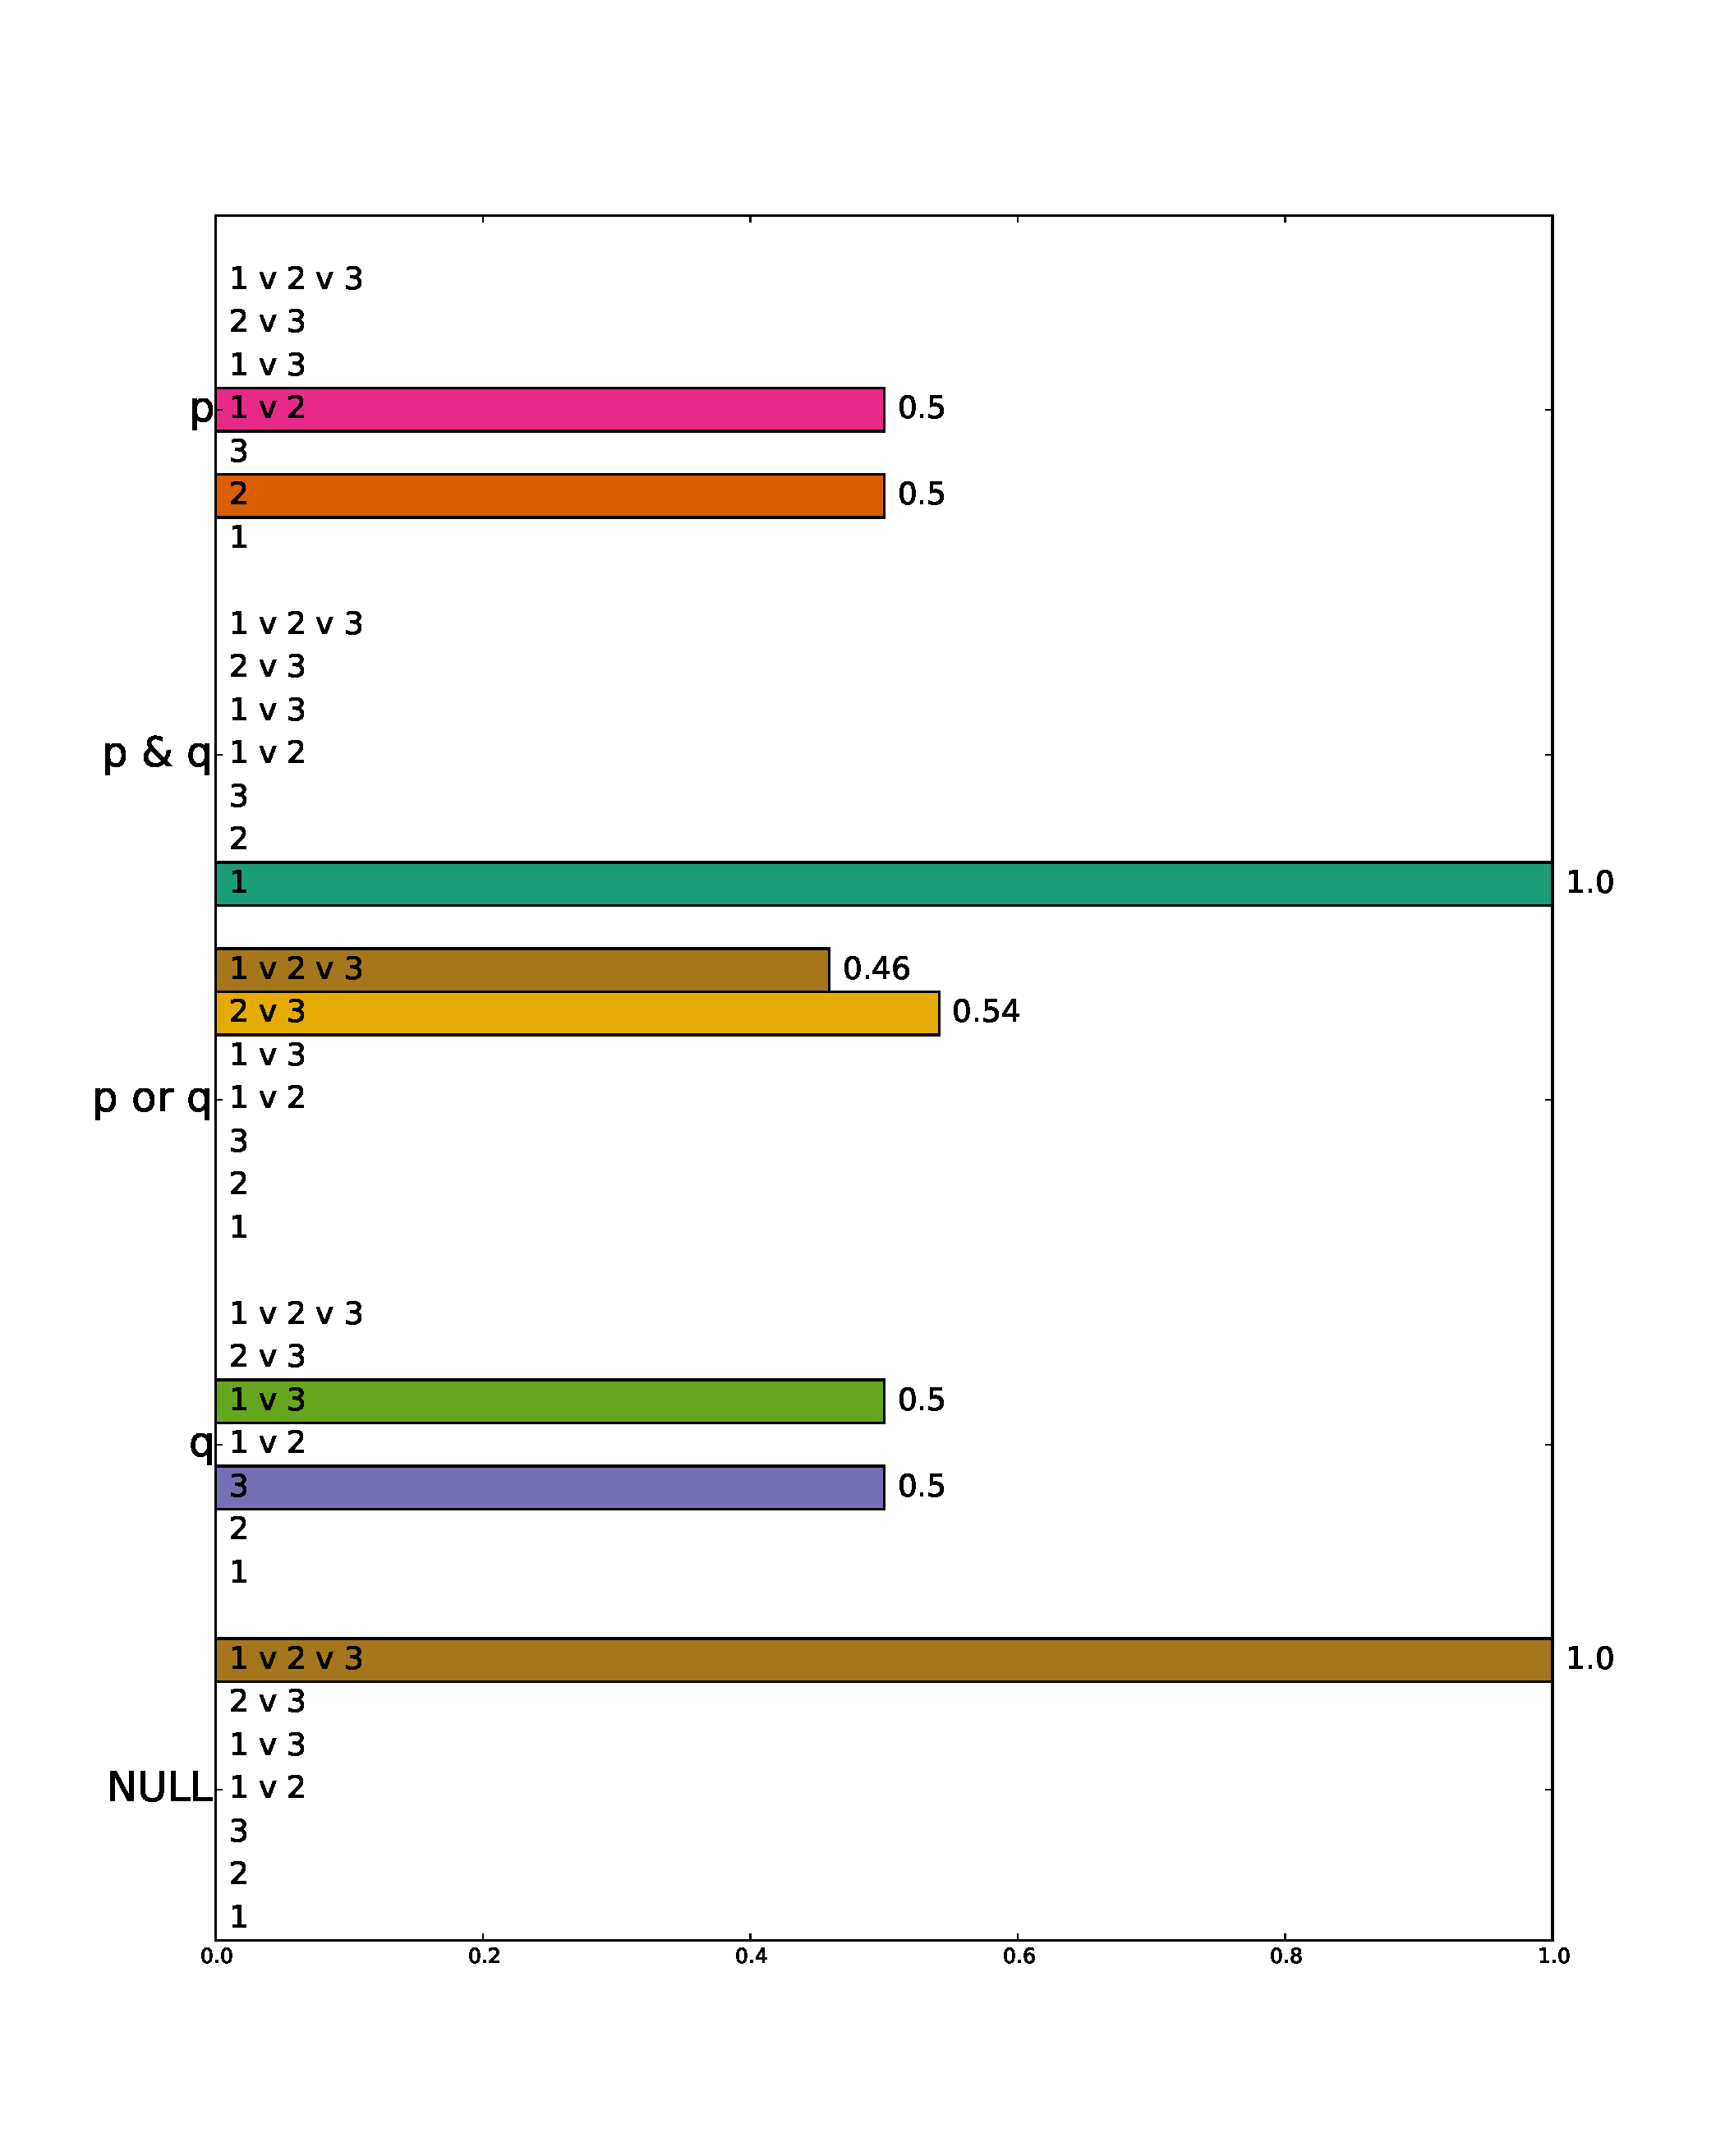
\includegraphics[width=1.2\textwidth]{fig/scalardisj-expertise-listener-marginalized}
  \end{examples}
\end{minipage}
\hfill
\begin{minipage}[c]{0.48\linewidth}
  \begin{examples}
  \item $\SpeakerK[3]$ summed over lexica
    
    \vspace{-4pt}

    $\mspace{-70mu}$
    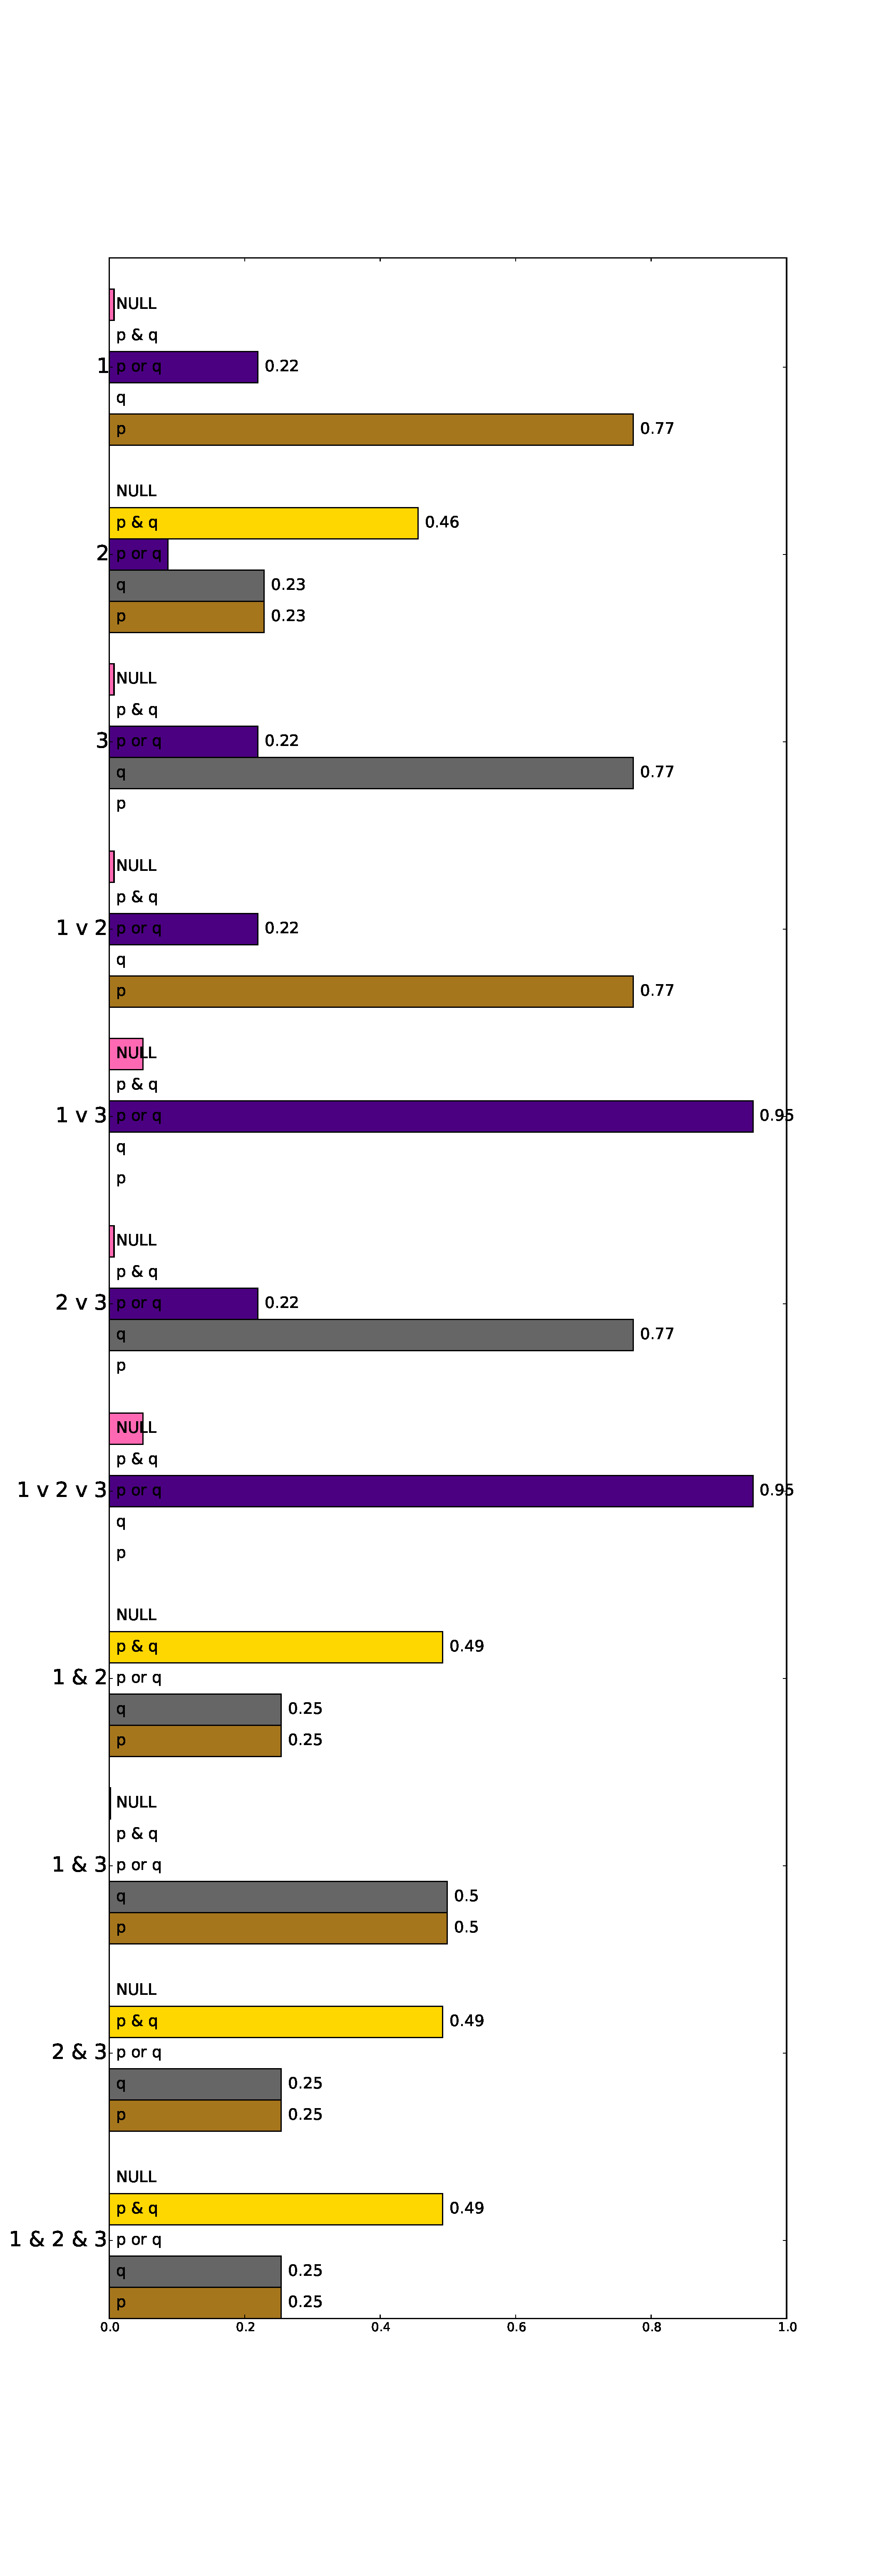
\includegraphics[width=1.2\textwidth]{fig/scalardisj-expertise-speaker-lexsum}
  \end{examples}
\end{minipage}

\begin{examples}
\item Summary of the above via max associations:

  \begin{minipage}[t]{0.45\linewidth}
    Listener

    \vspace{-2pt}
  
    $\begin{array}[t]{r @{ \ \Rightarrow \ } l}
      \toprule
      \text{Message} & \text{Inference} \\
      \midrule
      p &  w_{1}\\
      q & w_{3} \\
      p \word{ or } q & w_{1} \vee w_{3} \\
      \bottomrule
    \end{array}$
  \end{minipage}
  \hfill
  \begin{minipage}[t]{0.45\linewidth}
    Speaker

    \vspace{-2pt}

    $\begin{array}[t]{r @{ \ \Rightarrow \ } l}
      \toprule
      \text{Observation} & \text{Best message} \\
      \midrule
      w_{1} & p \\
      w_{2} & \set{p, q} \\
      w_{3} & q  \\      
      w_{1} \vee w_{3} & p \word{ or } q \\
      \bottomrule
    \end{array}$
  \end{minipage}    
\end{examples}

%=====================================================================

\section{Analysis}\label{sec:analysis}


Throughout, we
assume that the communcative setting is governed by a few overarching
principles: 

 communication about language is at least somewhat
important to the discourse participants; 

Contextual requirements: 

\begin{examples}
\item The speaker is mutually and publicly known to be an expert in
  the relevant domain.
  
\item The speaker is mutually and publicly known to believe the
  listener to be a non-expert in the relevant domain.
  
\item The speaker is mutually and publically known to have an
  interest in conveying information about the language itself,
  even if this communicative inefficiency in terms of the 
  information conveyed about the world.
\end{examples}

\begin{examples}
\item Throughout, let \word{X} be the unknown term.

\item From the listener's perspective, we are concerned to see when
  \word{A or X} gives rise to the inference that $\sem{A} \cap \sem{X}
  = \emptyset$ (Hurfordian reading) and when \word{A or X} gives rise
  to the inference that $\sem{A} = \sem{X}$ (definitional).
\end{examples}

\newcommand{\smallhurfordlex}[3]{
  \left[
    \begin{array}[c]{l@{ \ \mapsto \ }r l@{ \ \mapsto \ }r l@{ \ \mapsto \ }r}
      A & \set{#1} &
      B & \set{#2} &
      X & \set{#3}
    \end{array}
  \right]}

%=====================================================================

\subsection{Subsumptive disjunctions}\label{sec:analysis:subsumptive}

\begin{examples}
\item From the listener's perspective, we are concerned to see when
  \word{A or X} gives rise to the lexical inference that $\sem{A} \cap
  \sem{X} = \emptyset$. We assume that the overall meaning will be
  $\sem{A} \cup \sem{X}$, i.e., that the relevant information concerns
  just the lexical inference.

\item Here's a scenario in which the exclusivization inference arises:

  \begin{examples}
  \item $\States = \set{w_{1}, w_{2}, w_{3}}$;  $\Messages = \set{A, B, X}$
  \item $\Lex = [A \mapsto \set{w_{1}}, B \mapsto \set{w_{2}}, X \mapsto \set{w_{1}, w_{2}}]$
  \item Priors are flat. $\alpha = 2$; $\beta = 1$; $\gamma = 1$. Disjunction cost: $1$. $n = 3$. 
  \end{examples}

\item The listener's best guess inference, upon hearing \word{A or X},
  is that the speaker's state is $w_{1} \vee w_{2}$ and that the
  lexicon is the one where $A$ and $X$ are disjoint. Here's the joint
  probability table:
  \[
  \renewcommand{\arraystretch}{2}
  \begin{array}[c]{l r r r}
    \toprule
            & w_{1} & w_{2} & w_{1} \vee w_{2} \\
    \midrule
    \smallhurfordlex{w_{1}}{w_{2}}{w_{1}, w_{2}} & 0 & 0 & 0.16 \\
    \smallhurfordlex{w_{1}}{w_{2}}{w_{2}} & 0 & 0 & \graycell{0.47} \\
    \smallhurfordlex{w_{1}}{w_{2}}{w_{1}} & 0 & 0 & 0.38 \\
    \bottomrule
  \end{array}
  \]

\item The above parameters deliver the same result with the the
  lexicon size increased (same pattern: each lexical item denotes its
  own world and $X$ denotes the union of all the worlds). This is
  unwieldy to visualize, but the important thing is that the best
  lexicon is always a Hurfordian one. Here's the best lexical
  inference with five atomic messages and four atomic states:
  \[
  \left[
    \begin{array}[c]{l@{ \ \mapsto \ }l}
      A & \set{w_{1}} \\
      B & \set{w_{2}} \\
      C & \set{w_{3}} \\
      D & \set{w_{4}} \\
      X & \set{w_{2}, w_{3}, w_{4}}
    \end{array}
  \right]
  \]
  This is the `minimal' Hurfordian lexicon: the listener doesn't infer
  anything about $X$ except that it is disjoint from $A$.    
\end{examples}

%=====================================================================

\subsection{Definitional disjunctions}\label{sec:analysis:definitional}

\begin{examples}
\item From the listener's perspective, we are concerned to see when
  \word{A or X} is interpreted as equivalent to $\sem{A}$.

\item From the speaker's perspective, we want to know what happens
  when the speaker favors a lexicon in which $\sem{A}=\sem{X}$ and
  observes a state equivalent to the literal meaning of $\sem{A}$.
  When will such a speaker produce \word{A or X}.

\item Here's an example in which these two perspectives are
  complementary. To achieve it, we have to substantially raise
  $\alpha$ and $\beta$ and lower disjunction costs:

  \begin{examples}
  \item $\States = \set{w_{1}, w_{2}, w_{3}}$;  $\Messages = \set{A, B, X}$
  \item $\Lex = [A \mapsto \set{w_{1}}, B \mapsto \set{w_{2}}, X \mapsto \set{w_{1}, w_{2}}]$
  \item Priors are flat. $\alpha = 5$; $\beta = 7$; $\gamma = 1$. Disjunction cost: $0.01$. $n = 3$. 
  \end{examples}

\item The listener's best guess inference, upon hearing \word{A or X},
  is that the speaker's state is $w_{1} \vee w_{2}$ and that the
  lexicon is $\Lex_{1}$. Here's the joint probability table:
  \[
  \renewcommand{\arraystretch}{2}
  \begin{array}[c]{l r r r}
    \toprule
            & w_{1} & w_{2} & w_{1} \vee w_{2} \\
    \midrule
    \smallhurfordlex{w_{1}}{w_{2}}{w_{1}, w_{2}} & 0 & 0 & 0 \\
    \smallhurfordlex{w_{1}}{w_{2}}{w_{2}}        & 0 & 0 & 0 \\
    \smallhurfordlex{w_{1}}{w_{2}}{w_{1}}        & \graycell{0.88} & 0 & 0.12\\
    \bottomrule
  \end{array}
  \]

\item The above parameters deliver the same result with the the
  lexicon size increased. Here's the best lexical inference with five
  atomic messages and four atomic states --- in this way, the 
  listener has learned that $A$ and $X$ are synonymous:
  \[
  \left[
    \begin{array}[c]{l@{ \ \mapsto \ }l}
      A & \set{w_{1}} \\
      B & \set{w_{2}} \\
      C & \set{w_{3}} \\
      D & \set{w_{4}} \\
      X & \set{w_{1}}
    \end{array}
  \right]
  \]  

\item If we assume that the unknown term has an atomic meaning, then
  we can strengthen the inference (and generate it under a wider range
  of parameters settings).  Under these circumstances, the meaning of
  the known disjunct serves as a \emph{focal point} that the speaker
  and listener can coordinate on for the meaning of the unknown word.
\end{examples}

%=====================================================================

\subsection{Characterization}\label{sec:analysis:characterization}

\begin{examples}
\item The basic characterization is that definitional reading arise
  when disjunction costs are low and $\beta$ is high. Conversely,
  Hurfordian reading arise when disjunction cost are high and $\alpha$
  and $\beta$ are relatively close.
  
\item The intuition: where costs are high, the disjunction has to be
  justified. Letting the two terms overlap reduces the justification,
  whereas exclusivizing provides justification. In other words, the
  apparently undue prolixity of the disjunction (the more general term
  would seem to suffice!) generates an inference that we observe in
  the lexical inferences.
  
\item However, this needs to be qualified by the speaker's desire to
  communicate about the lexicon. If $\beta$ is high, then it might be
  worth paying the disjunction costs for the sake of teaching the
  listener about the lexicon, even if this involves a huge penalty in
  terms of informativity (since definitional readings convey only
  a single term's worth of information).

\item Earlier, we gave this charaterization of the contextual
  requirements for definitional readings. The boldfaced phrases
  connect these ideas with our model.

  \begin{examples}
  \item The speaker is mutually and publicly known to be an expert in
    the relevant domain. \textbf{The speaker observes a lexicon--state
      pair, and the listener seeks to figure out which one, which
      entails moving towards the speaker's lexicon.}      

  \item The speaker is mutually and publicly known to believe the
    listener to be a non-expert in the relevant domain.  \textbf{The
      speaker has lexical uncertainty --- it doesn't assume a lexicon
      but rather tries to infer one.}

  \item The speaker is mutually and publically known to have an
    interest in conveying information about the language itself, even
    if this communicative inefficiency in terms of the information
    conveyed about the world.  \textbf{High $\beta$, low disjunction
      costs.}
  \end{examples}

\item Additionally, the secondary nature of the definitional
  information (as compared with \word{oenophile means wine lover}) is
  captured by the fact that the inference is primarily about the
  lexicon, rather than about the information conveyed --- after all,
  absence the lexical inference, \word{A} would have done the same
  work with lower costs.

\item Hurfordian readings arise in a much wider range of parameters
  settings, that is contexts, because they survive high definitional
  costs are long as they can be justified.

\item Definitional readings exist mainly in the space of low
  disjunction and high $\beta$. This is more rarefied. We believe this
  is reflected in the data: definitional readings are relatively
  infrequent and delicate.

\item Here's a plot that does a good job of conveying the above.  It's
  for a relatively large lexicon: five atomic lexical items and five
  atomic states. (Smaller examples can be hard to interpret, since the
  model's overall pressure to achieve separating equilibria can
  create associations that we wouldn't expect to see in a more complex
  setting like, well, English.) The x-axis is $\log(\beta/\alpha)$, so
  $0.$ marks the points where $\beta = \alpha$. The y-axis is 
  the cost of disjunction (assuming $\gamma=1.0$).

  $\mspace{-80mu}$
  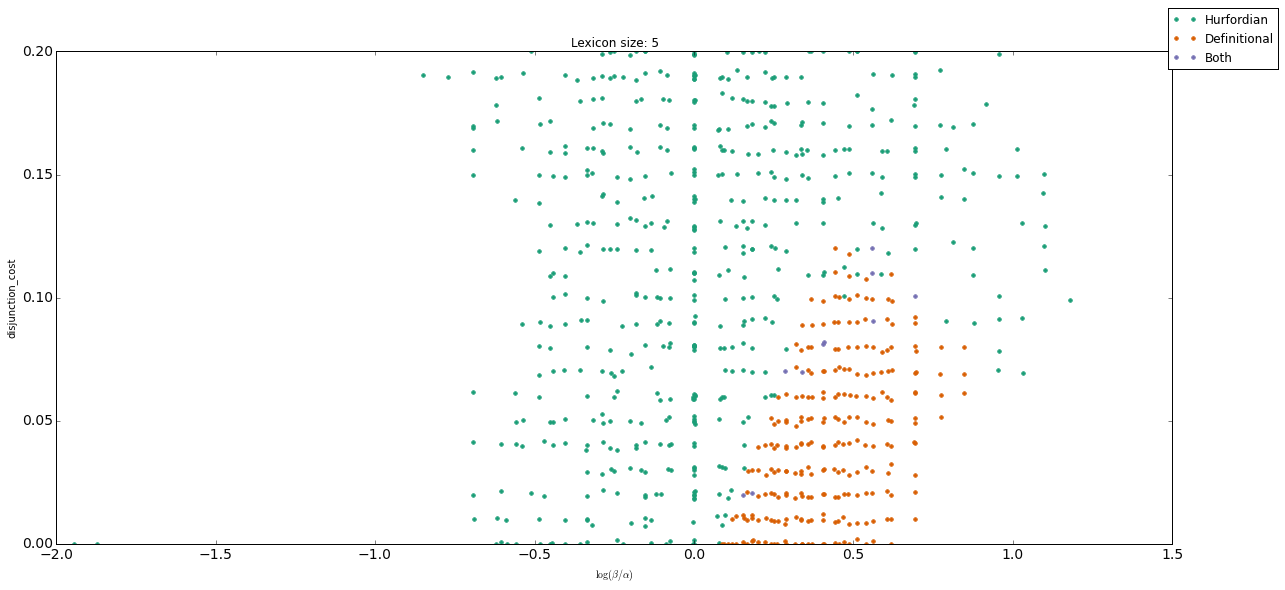
\includegraphics[width=1.2\textwidth]{fig/lex5-alpha-beta-gamma}

\end{examples}

%=====================================================================

\bibliographystyle{apalike}
\bibliography{levy-potts-pragdisj-bib}

\end{document}


